%% ============================================================
%% main.tex  —  LifeLink AI  IEEE MedAI 2026 Regular Paper
%% Compile:  pdflatex -> bibtex -> pdflatex -> pdflatex
%% ============================================================
\documentclass[conference]{IEEEtran}

%% ---------- packages ----------
\usepackage[T1]{fontenc}
\usepackage[utf8]{inputenc}
\usepackage{amsmath,amssymb}
\usepackage{graphicx}
\usepackage{booktabs}
\usepackage{multirow}
\usepackage{array}
\usepackage{url}
\usepackage{cite}
\usepackage{hyperref}

\hypersetup{
  hidelinks,
  pdftitle={LifeLink AI: A Trustworthy Hybrid Architecture for
            Real-Time Emergency Blood Matching},
  pdfauthor={Shivang Mishra et al.},
}

%% ============================================================
\begin{document}

\title{LifeLink AI: A Trustworthy Hybrid Clinical Decision-Support
Architecture for Real-Time Emergency Blood Matching in Digital and
Precise Medicine}

\author{%
  \IEEEauthorblockN{Shivang Mishra, Lakshya Sahu, Kushagra Bhargava,
                    Anshul, Archisha Nigam, Mokshi Jain}
  \IEEEauthorblockA{VIT Bhopal University, Bhopal, India}
}

\maketitle

%% ============================================================
\begin{abstract}
Emergency blood provision during acute haemorrhagic trauma, perioperative
crises, and obstetric complications demands sub-minute coordination under
uncompromising patient-safety constraints. Conventional procurement relies
on fragmented telephonic cascades and static web directories, introducing
latencies of 20--60 minutes that substantially elevate mortality within
the \emph{golden hour}. This paper presents \textbf{LifeLink AI}, a
trustworthy hybrid clinical decision-support architecture for real-time
emergency blood matching within the paradigm of Digital and Precise
Medicine. The system implements a formally defined \textbf{two-layer
safety contract}: Layer~1 enforces an immunohematological verification
gate---an O(1) ABO/Rh compatibility look-up, a mandatory 56-day
whole-blood recovery cooldown, and a minimum 45\,kg body-mass
constraint---that is computationally isolated from any machine-learning
component. Layer~2 applies a calibrated logistic-regression
donor-response propensity model, whose sole purpose is to rank
Layer-1-qualified candidates by their estimated willingness to respond
to an emergency alert. The propensity model is trained on the UCI Blood
Transfusion Service Center benchmark (748 records, 5-fold stratified
cross-validation) and achieves ROC-AUC\,=\,0.7521, Recall\,=\,0.7528,
Precision\,=\,0.3907, F1\,=\,0.5144, and Brier Score\,=\,0.2055.
The end-to-end platform is containerised across six microservices and
validated by 56 automated integration tests (100\% pass rate). System
benchmarking yields mean matching latencies of 47.2\,ms (AI~path)
and 12.4\,ms (deterministic fallback). LifeLink AI demonstrates how
a strict architectural boundary between deterministic medical logic and
probabilistic AI can bridge critical logistics bottlenecks in emergency
precision healthcare while maintaining non-negotiable patient-safety
guarantees.
\end{abstract}

\begin{IEEEkeywords}
Digital and precise medicine; trustworthy AI; clinical decision support;
emergency blood matching; immunohematology; donor response propensity;
hybrid architecture; logistic regression; RFM model; microservices.
\end{IEEEkeywords}

%% ============================================================
\section{Introduction}

Haemorrhagic shock from traumatic injury, postpartum haemorrhage, or
major surgery is a leading cause of preventable mortality. Clinical
evidence shows that every ten-minute delay in cross-match-compatible
transfusion significantly increases multiorgan failure risk
\cite{cotton2018,cole2019}. The WHO estimates 118.5 million annual
blood donations globally, yet profound logistical inequities persist
\cite{who2022}. In India, annual demand approaches 14 million units;
the challenge is a coordination failure rather than an absolute
shortage~\cite{nbtc2022}.

Current emergency blood procurement suffers from three structural
defects: \emph{(i)} uncoordinated telephonic cascades across blood
banks and donor lists, consuming 20--60 minutes per requisition;
\emph{(ii)} static directories with no real-time inventory visibility,
causing high rejection rates; and \emph{(iii)} undifferentiated donor
lists that ignore recency, frequency, and proximity, wasting critical
minutes on donors unlikely to respond.

Introducing AI into emergency medicine also creates medicolegal risk:
an ABO-incompatible recommendation can cause acute intravascular
haemolysis and death. LifeLink AI resolves this tension through a
strict architectural boundary: biological compatibility and statutory
eligibility are determined exclusively by deterministic medical logic,
while machine learning operates only as an advisory ranking tool.

\textbf{Research Contributions:}
\begin{enumerate}
  \item \emph{Two-Layer Safety Contract}---a formalised pattern that
        mathematically isolates zero-tolerance medical invariants from
        probabilistic AI across containerised network boundaries.
  \item \emph{Hybrid Composite Scoring}---an interpretable ranking
        function integrating compatibility quality, PostGIS geospatial
        proximity, operational availability, and AI response propensity.
  \item \emph{Calibrated ML Propensity Model}---balanced logistic
        regression trained on the UCI BTSC benchmark, prioritising
        clinical recall (0.7528) over raw accuracy.
  \item \emph{Production-Grade Validation}---56 automated integration
        tests at 100\% pass rate, sub-100\,ms latencies, and
        pessimistic \texttt{SELECT\ldots FOR UPDATE} concurrency locking.
  \item \emph{ReBAC Governance}---a 7-role multi-tenant access control
        model with immutable audit logging.
\end{enumerate}

%% ============================================================
\section{Related Work}

\subsection{Blood Supply Chain Logistics}
Blood product management has been studied as a perishable inventory
routing problem. Stanger \emph{et~al.}~\cite{stanger2012} identified
fragmented inventory visibility as the primary driver of blood
wastage and acute shortages. Heitmiller \emph{et~al.}~\cite{heitmiller2008}
showed that algorithmic ordering guidelines reduced unnecessary
cross-matches by 42\%. IoT and RFID-based cold-chain monitoring
\cite{roy2021} addresses facility-level traceability, but not
real-time multi-facility emergency coordination. India's \emph{e-Rakt
Kosh}~\cite{eraktkosh2020} functions as a passive administrative
registry without automated spatial matching or predictive donor modeling.

\subsection{Machine Learning in Donor Behaviour}
Yeh \emph{et~al.}~\cite{yeh2009} established the RFM (Recency,
Frequency, Monetary) framework for blood donation, demonstrating
that recent and frequent donors exhibit measurably higher future
response propensity. Gilliss \emph{et~al.}~\cite{gilliss2021}
confirmed that timely, targeted communication is a dominant
predictor of donor retention. Meta-analyses~\cite{baesens2003}
show that regularised logistic regression matches or exceeds
ensemble classifiers on small behavioral feature sets while
providing superior probability calibration and intrinsic
interpretability---properties critical in safety-critical healthcare.

\subsection{Trustworthy AI in Healthcare}
Rudin~\cite{rudin2019} argued that interpretable models should be
preferred over black-box alternatives in high-stakes decisions.
Doshi-Velez and Kim~\cite{doshivelez2017} formalised the distinction
between \emph{intrinsic} interpretability (model equations are
self-explanatory) and post-hoc surrogates (LIME, SHAP). The EU
High-Level Expert Group on AI~\cite{eu_hleg2019} and the IEEE
Ethically Aligned Design~\cite{ieee_ead2019} mandate transparency,
non-maleficence, robustness, and human oversight---all operationalised
in LifeLink AI's architecture. The EU AI Act~\cite{eu_ai_act2021}
classifies medical decision-support systems as high-risk, requiring
mandatory logging and human oversight.

\textbf{Positioning.} Table~\ref{tab:comparison} contrasts LifeLink AI
with representative prior systems across six critical dimensions.
LifeLink AI is the only system combining deterministic O(1) compatibility
guarantees, intrinsically interpretable AI ranking, a resilient
three-level fallback, and pessimistic concurrency control.

\begin{table}[t]
  \centering
  \caption{Comparison of Blood Coordination System Architectures}
  \label{tab:comparison}
  \setlength{\tabcolsep}{3pt}
  \renewcommand{\arraystretch}{1.1}
  \begin{tabular}{@{}p{1.6cm}p{1.4cm}p{1.4cm}p{1.6cm}@{}}
    \toprule
    \textbf{Dimension} & \textbf{Static Reg.} & \textbf{Pure ML} & \textbf{LifeLink AI} \\
    \midrule
    Compatibility  & Manual         & Probabilistic      & Det.\ O(1) Gate \\
    Donor Priority & FIFO           & Black-Box          & Calibrated LR   \\
    Explainability & N/A            & Post-Hoc           & Intrinsic       \\
    Fallback       & Manual         & Unhandled          & 3-Level Chain   \\
    Concurrency    & None           & None               & FOR UPDATE Lock \\
    Audit Trail    & None           & Informal           & Immutable Ledger\\
    \bottomrule
  \end{tabular}
\end{table}

%% ============================================================
\section{Problem Formulation and System Model}

\subsection{Emergency Request}
A blood requisition is a typed tuple:
\begin{equation}
  E = \bigl(\mathrm{req\_id},\;\beta_\mathrm{rec},\;\gamma,\;
            u_\mathrm{req},\;\lambda_\mathrm{dest},\;\omega,\;t_0\bigr)
\end{equation}
where $\beta_\mathrm{rec}\!\in\!\mathcal{B}=\{\text{O}\pm,
\text{A}\pm,\text{B}\pm,\text{AB}\pm\}$ is the recipient blood group;
$\gamma\!\in\!\{\text{Whole Blood, RBC, Plasma, Platelets}\}$ is the
prescribed component; $u_\mathrm{req}\!\in\![1,20]$ is the requested
units; $\lambda_\mathrm{dest}=(\phi,\psi)$ are WGS-84 coordinates;
$\omega\!\in\!\{\text{LOW,MED,HIGH,CRITICAL}\}$ is urgency;
and $t_0$ is the UTC submission timestamp.

\subsection{Candidate Pools}
Registered voluntary donors $\Omega_D=\{d_1,\ldots,d_N\}$ and
licensed blood banks $\Omega_K=\{k_1,\ldots,k_M\}$ are indexed
by PostGIS GiST geometry columns (SRID~4326). Each donor is
parameterised by $d_i=(\beta_i,w_i,a_i,e_i,\lambda_i,t_\mathrm{last},
F_i,T_i)$ where $w_i$ (kg) is body mass, $a_i,e_i\!\in\!\{0,1\}$ are
availability and eligibility flags, and $(F_i,T_i)$ are the RFM
behavioral features. Table~\ref{tab:notation} summarises key notation.

\begin{table}[t]
  \centering
  \caption{Key Mathematical Notation}
  \label{tab:notation}
  \setlength{\tabcolsep}{3pt}
  \renewcommand{\arraystretch}{1.05}
  \begin{tabular}{@{}lll@{}}
    \toprule
    \textbf{Symbol} & \textbf{Domain} & \textbf{Meaning} \\
    \midrule
    $\beta_\mathrm{rec},\beta_\mathrm{don}$ & $\mathcal{B}$ & Recipient/donor ABO/Rh group \\
    $\lambda=(\phi,\psi)$ & WGS-84 & Geospatial coordinates \\
    $d_\mathrm{hav}(\lambda_1,\lambda_2)$ & km & Haversine great-circle distance \\
    $R_\mathrm{search}$ & \{15,25,50,100\}\,km & Active spatial radius \\
    $\Delta t_\mathrm{cool}$ & $\geq$56\,days & Recovery cooldown constraint \\
    $P_\mathrm{ML}$ & $[0,1]$ & Logistic regression propensity \\
    $P_\mathrm{geo}$ & $[0,1]$ & Linear spatial proximity decay \\
    $S_\mathrm{donor},S_\mathrm{bb}$ & $[0,1]$ & Composite ranking scores \\
    $\alpha_1,\alpha_0$ & $\mathbb{R}^+$ & Balanced inverse class weights \\
    \bottomrule
  \end{tabular}
\end{table}

%% ============================================================
\section{Proposed Methodology and Safety Architecture}

\subsection{The Two-Layer Safety Contract}

The central design principle of LifeLink AI is a strict, architecturally
enforced separation of concerns illustrated in Fig.~\ref{fig:arch}.
\emph{Layer~1} applies deterministic medical logic that cannot be
overridden by any probabilistic component. \emph{Layer~2} applies AI
exclusively to the operational ranking of Layer-1-qualified candidates.
These layers occupy different Docker containers and communicate only
through defined API contracts.

\begin{figure}[t]
  \centering
  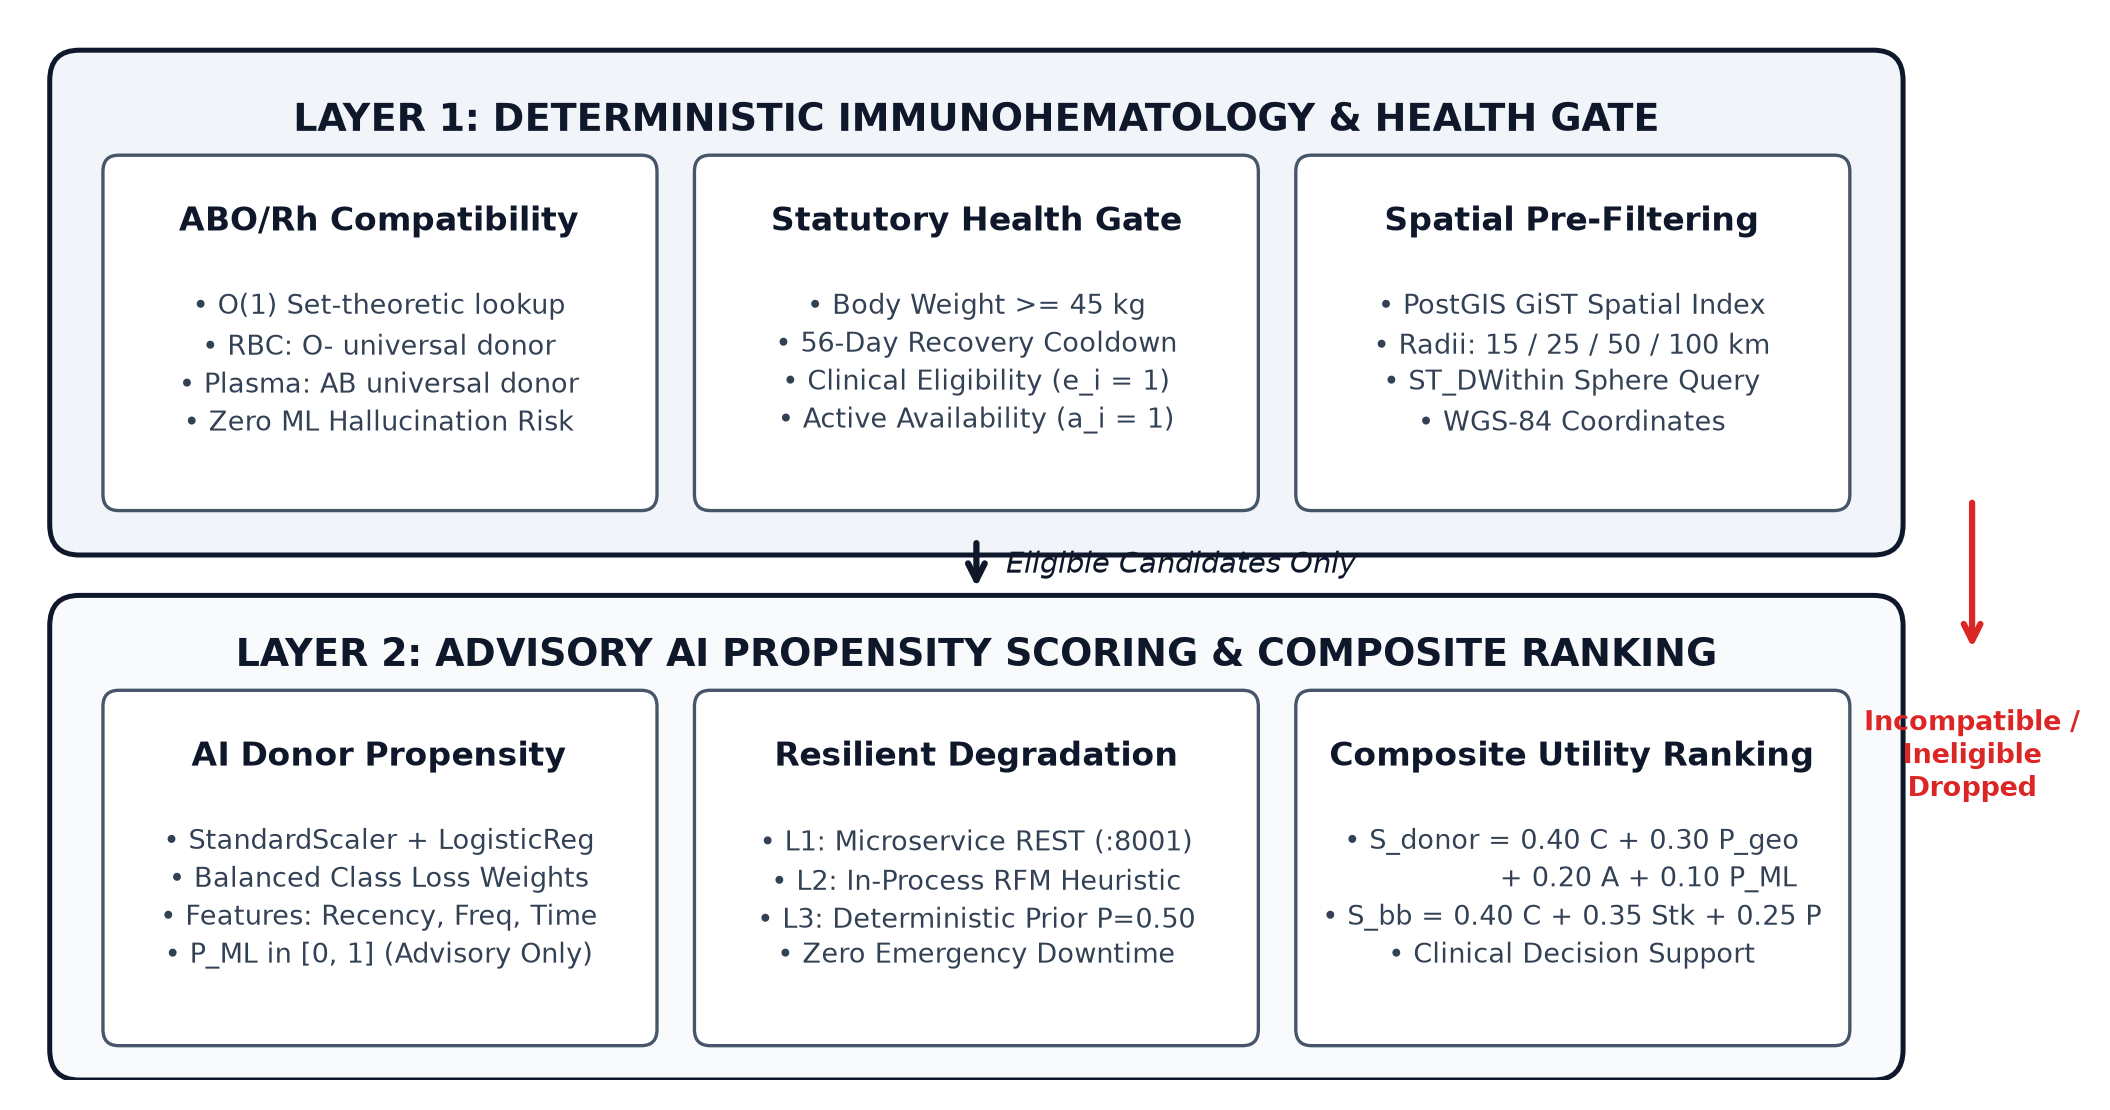
\includegraphics[width=\columnwidth]{figures/lifelink_architecture.png}
  \caption{LifeLink AI two-layer safety contract: Layer~1 enforces
  deterministic immunohematological and statutory eligibility gates;
  Layer~2 applies calibrated AI propensity scoring for advisory ranking
  only. Medical safety decisions are exclusively Layer-1 outputs.}
  \label{fig:arch}
\end{figure}

\subsection{Layer 1: Deterministic Medical Compatibility Gate}

Immunohematological compatibility is an immutable biological law:
administering ABO-incompatible blood can cause fatal intravascular
haemolysis. The compatibility gate is implemented as a pure-Python,
ML-free O(1) dictionary look-up in \texttt{backend/app/core/medical.py}.
For Whole Blood and Packed Red Blood Cells (PRBC):
\begin{equation}
  C_\mathrm{RBC}(\beta_\mathrm{rec})
    = \bigl\{\,\beta_\mathrm{don}\in\mathcal{B}
      \mid \text{donor RBC compatible with }\beta_\mathrm{rec}\bigr\}
\end{equation}
For Fresh Frozen Plasma (FFP), compatibility inverts to the donor
antibody profile ($\text{AB}\!\to\!$universal donor):
\begin{equation}
  C_\mathrm{Plasma}(\beta_\mathrm{rec})
    = \bigl\{\,\beta_\mathrm{don}\in\mathcal{B}
      \mid \text{donor plasma compatible with }\beta_\mathrm{rec}\bigr\}
\end{equation}
A donor $d_i$ passes Layer~1 if and only if all five conditions hold:
\begin{equation}
  \mathrm{Gate}(d_i) \;=\;
    [\beta_i\!\in\!C] \;\wedge\; [e_i{=}1] \;\wedge\; [a_i{=}1]
    \;\wedge\; [\Delta t_\mathrm{cool}\!\geq\!56] \;\wedge\; [w_i\!\geq\!45]
\end{equation}
The 56-day cooldown is WHO-mandated; the 45\,kg floor is enforced by
both application logic and a PostgreSQL \texttt{CHECK} constraint.
Donors failing any single predicate are unconditionally excluded before
any scoring computation.

\subsection{Layer 2: Multi-Criteria Composite Ranking}

Candidates surviving Layer~1 are ranked by a composite score. Spatial
proximity decays linearly over the active PostGIS search radius:
\begin{equation}
  P_\mathrm{geo} = \max\!\bigl(0,\;1 - d_\mathrm{hav}/R_\mathrm{search}\bigr)
\end{equation}
The composite donor score integrates four orthogonal signals:
\begin{equation}
  S_\mathrm{donor} =
    0.40\,C_\mathrm{score} + 0.30\,P_\mathrm{geo}
    + 0.20\,A_\mathrm{score} + 0.10\,P_\mathrm{ML}
  \label{eq:sdonor}
\end{equation}
where $C_\mathrm{score}=1.0$ for exact ABO/Rh match (0.8 for universal
compatible); $A_\mathrm{score}=1.0$ for available donors; and
$P_\mathrm{ML}$ is the calibrated propensity probability. For blood
banks, stock sufficiency replaces propensity:
\begin{equation}
  S_\mathrm{bb} =
    0.40\,C_\mathrm{score} + 0.35\,\mathrm{Stock}_\mathrm{score}
    + 0.25\,P_\mathrm{geo}
  \label{eq:sbb}
\end{equation}
where $\mathrm{Stock}_\mathrm{score}=\min(1,\,u_\mathrm{avail}/u_\mathrm{req})$.
The weight assignments reflect deliberate clinical priorities:
compatibility (0.40) and proximity (0.30) dominate because they most
directly determine the feasibility and speed of procurement; AI propensity
(0.10) provides evidence-based uplift without overriding clinical factors.

%% ============================================================
\section{System Architecture and Implementation}

\subsection{Microservice Topology}
LifeLink AI is containerised across six isolated Docker services:
\texttt{lifelink-nginx} (port~80, reverse proxy),
\texttt{lifelink-frontend} (port~3000, Next.js~14.2.5),
\texttt{lifelink-backend} (port~8000, FastAPI~0.111.1 on Python~3.11),
\texttt{lifelink-ai-service} (port~8001, scikit-learn~1.5.1 inference),
\texttt{lifelink-postgres} (port~5432, PostgreSQL~15 + PostGIS~3.3),
and \texttt{lifelink-redis} (port~6379, Redis~7). All inter-service
traffic runs on an internal Docker bridge network; only Nginx is
externally exposed. The AI service occupies its own isolated container,
enforcing the Layer~1/Layer~2 separation at the process boundary.

\subsection{Relational Schema and Concurrency Control}
Eleven relational tables manage platform state under migration control.
Spatial attributes are stored as native PostGIS geometry objects
(SRID~4326) indexed with GiST, enabling O(\(\log N\)) radius queries
via \texttt{ST\_DWithin}. The \texttt{inventory\_history} table is
an append-only immutable audit ledger (UPDATE/DELETE disallowed at the
database role level).

Under concurrent emergency load, multiple hospitals may simultaneously
request the same rare blood group. \textbf{Pessimistic row-level locking}
via \texttt{SELECT\ldots FOR UPDATE} serialises concurrent reservation
attempts: the locked transaction increments \texttt{units\_reserved},
validates sufficiency, commits atomically, and writes an inventory
audit record---preventing double-allocation without optimistic retry
loops.

\subsection{Security and Access Control}
A seven-role \emph{Relationship-Based Access Control} (ReBAC) hierarchy
(SUPER\_ADMIN $\to$ ADMIN $\to$ \{HOSPITAL\_ADMIN, BB\_MANAGER\}
$\to$ staff $\to$ DONOR) is enforced at three layers: JWT HMAC-SHA256
signature verification (30-min access, 7-day refresh), FastAPI
dependency injection validating role and tenancy, and SQLAlchemy query
filters scoping all data to the requesting institution. Cross-tenant
access is rejected with HTTP~403 before any database query executes.
Patient PII on tracking portals is protected by cryptographic UUID tokens.

\subsection{Facility Verification Model}
Hospitals and blood banks register statutory identifiers, license dates,
and certificate PDFs. \emph{Design boundary}: the platform stores these
documents for administrative governance review; it does \emph{not}
validate licenses against live government APIs (CDSCO/SBTC registries).
This decouples the one-time institutional onboarding trust process from
the real-time emergency matching pipeline.

%% ============================================================
\section{AI Donor Response Propensity Model}

\subsection{Role and Clinical Boundaries}
The AI component is an \textbf{advisory response propensity estimator}.
Its sole function is to estimate the conditional probability that a
Layer-1-qualified donor will accept an emergency alert and travel to
the collection center. It does \emph{not} determine blood compatibility,
assess medical eligibility, diagnose patients, or initiate dispatch.
The AI service receives only behavioral features $(R, F, T)$ and returns
only $P_\mathrm{ML}\in[0,1]$; it cannot read or modify blood group data.

\subsection{Dataset and Feature Engineering}
The model is trained on the UCI Blood Transfusion Service Center (BTSC)
benchmark~\cite{yeh2009} (OpenML ID~1464, CC~BY~4.0): $N=748$ anonymised
donor records from Hsin-Chu, Taiwan, with $N_+{=}178$ (23.8\%) positive
and $N_-{=}570$ (76.2\%) negative instances---a 3.2:1 class imbalance.

The dataset provides four features: Recency~($R$), Frequency~($F$),
Monetary~($M{=}250F$), Time~($T$). Statistical analysis confirms exact
collinearity $M=250F$ (Pearson $r=1.000$); retaining $M$ would produce
a singular Gram matrix. Accordingly, $M$ is pruned, yielding the
three-dimensional feature vector $\mathbf{x}=[R,F,T]^\top\in\mathbb{R}^3$.

\subsection{Model Architecture and Training}
Raw features are standardised via \texttt{StandardScaler} to zero mean
and unit variance:
\begin{equation}
  \mathbf{x}_\mathrm{std} = \boldsymbol{\Sigma}^{-1/2}(\mathbf{x}-\boldsymbol{\mu})
\end{equation}
Donor response propensity is then modelled by binary logistic regression:
\begin{equation}
  P(y{=}1\mid\mathbf{x})
    = \sigma\!\bigl(\mathbf{w}^\top\mathbf{x}_\mathrm{std}+b\bigr)
    = \frac{1}{1+e^{-(\mathbf{w}^\top\mathbf{x}_\mathrm{std}+b)}}
\end{equation}
To address class imbalance, the loss incorporates balanced inverse
class-frequency weights:
\begin{equation}
  \mathcal{L}(\mathbf{w},b)
    = -\frac{1}{N}\sum_{i=1}^{N}\!\Bigl[
        \alpha_1 y_i\log p_i
        + \alpha_0(1{-}y_i)\log(1{-}p_i)
      \Bigr]
      + \frac{\lambda}{2}\|\mathbf{w}\|_2^2
\end{equation}
\begin{equation}
  \alpha_1 = \frac{N}{2N_+} = 2.101,\qquad
  \alpha_0 = \frac{N}{2N_-} = 0.656
\end{equation}
where $\lambda=1/C$, $C=1.0$. The $\alpha_1>1$ weight penalises False
Negatives (missing a willing donor) more heavily than False Positives
(spurious alerts), reflecting the asymmetric clinical cost in emergency
dispatch. Optimisation uses the L-BFGS quasi-Newton algorithm.

\subsection{Three-Level Resilient Fallback}
To guarantee uninterrupted emergency operations under infrastructure
failures, LifeLink AI implements three degradation levels:
\textbf{(1)~Primary}: full calibrated logistic regression via the AI
microservice (port~8001);
\textbf{(2)~Secondary} (service reachable but model fails): closed-form
RFM heuristic executed in-process:
\begin{equation}
  P_\mathrm{fb} = \min\!\bigl(0.95,\;\max\!\bigl(0.05,\;
    0.40 + \max(0,\,0.35{-}0.01R) + \min(0.25,\,0.05F)\bigr)\bigr)
\end{equation}
\textbf{(3)~Tertiary} (microservice unreachable): backend assigns
neutral prior $P_\mathrm{ML}{=}0.50$ and records
\texttt{model\_version=`deterministic-fallback'} in the audit log. The
matching pipeline continues in all three levels, ensuring emergency
dispatch is never halted by AI infrastructure failure.

%% ============================================================
\section{Experimental Setup and Results}

\subsection{Evaluation Scope}
We explicitly distinguish three evaluation categories:
\emph{(i)}~\textbf{ML Model Evaluation}: offline 5-fold Stratified
Cross-Validation (SKF-CV) on the UCI BTSC benchmark;
\emph{(ii)}~\textbf{Software Engineering Verification}: automated
integration tests on live PostgreSQL~15 + Redis~7 instances in
Docker Compose;
\emph{(iii)}~\textbf{Clinical Validation}: \emph{not performed in this
study}. LifeLink AI is a research prototype that has not undergone
prospective clinical trials or regulatory clearance. Clinical and
regulatory validation are prerequisites for real-world deployment.

\subsection{ML Model Performance}
5-fold Stratified Cross-Validation ($K{=}5$, shuffle=True,
random\_state=42) preserves the 23.8\%/76.2\% class distribution
across all folds. The StandardScaler is fit only on training folds and
applied to test folds, preventing data leakage. Table~\ref{tab:ml}
presents out-of-fold performance metrics.

\begin{table}[t]
  \centering
  \caption{Donor Propensity Model: 5-Fold Stratified CV Results
           ($N{=}748$)}
  \label{tab:ml}
  \setlength{\tabcolsep}{3pt}
  \renewcommand{\arraystretch}{1.1}
  \begin{tabular}{@{}lcc@{}}
    \toprule
    \textbf{Metric} & \textbf{Value} & \textbf{Clinical Interpretation} \\
    \midrule
    Accuracy     & 0.6618 & Below majority baseline (76.2\%), expected under balanced weighting \\
    Precision    & 0.3907 & 39.1\% of alerted donors are willing responders \\
    Recall       & 0.7528 & 75.3\% of willing donors correctly identified \\
    F1-Score     & 0.5144 & Harmonic balance under 3.2:1 class imbalance \\
    ROC-AUC      & 0.7521 & Robust discrimination ($>$0.75); 0.50 = random \\
    PR-AUC       & 0.5028 & 2.1$\times$ improvement over naive baseline (0.238) \\
    Brier Score  & 0.2055 & Well-calibrated ($<$0.25 reference) \\
    \bottomrule
  \end{tabular}
\end{table}

\textbf{Analysis.} The balanced weighting deliberately prioritises
Recall over Precision because a False Negative (missing a willing
donor) directly threatens patient survival, while a False Positive
(an unnecessary alert) causes minor notification friction. The model
correctly identifies 134 of 178 willing donors (75.3\%). The PR-AUC
of 0.5028 is 2.1$\times$ the naive positive-class baseline (0.238),
confirming genuine discriminative value. The Brier score of 0.2055
validates that the probability estimates are well-calibrated for use
as a propensity signal in the composite ranking score
(Eq.~\ref{eq:sdonor}). Preliminary experiments with random forest and
gradient-boosted classifiers yielded ROC-AUC values of 0.74--0.76---a
marginal gain over logistic regression that does not justify the loss of
intrinsic interpretability in a safety-critical context~\cite{rudin2019}.

\subsection{Integration Test Suite}
Table~\ref{tab:tests} summarises the 56-test integration suite executed
against live services. All 56 tests pass (100\% success rate).

\begin{table}[t]
  \centering
  \caption{Integration Test Suite Summary (56/56 Pass)}
  \label{tab:tests}
  \setlength{\tabcolsep}{3pt}
  \renewcommand{\arraystretch}{1.1}
  \begin{tabular}{@{}lcp{3.3cm}@{}}
    \toprule
    \textbf{Test Domain} & \textbf{Count} & \textbf{Key Invariants} \\
    \midrule
    Auth.\ \& ReBAC        & 8 & JWT issuance, 7-role bounds, cross-tenant 403 \\
    Donor \& Health Gate   & 7 & 56-day cooldown, weight CHECK constraint \\
    Hospital Operations    & 6 & Emergency intake, coordinate storage \\
    Blood Bank Inventory   & 6 & Stock mgmt, certificate persistence \\
    Inventory Concurrency  & 7 & FOR UPDATE locking, double-allocation prevention \\
    Matching Pipeline      & 8 & Layer-1 gate, AI scoring, HTTP-503 fallback \\
    Emergency Lifecycle    & 7 & PENDING$\to$MATCHING$\to$FULFILLED transitions \\
    Admin Governance       & 4 & Certificate review, facility activation \\
    End-to-End             & 3 & Full cross-service dispatch flows \\
    \midrule
    \textbf{Total}         & \textbf{56} & \textbf{56/56 Passing (100\%)} \\
    \bottomrule
  \end{tabular}
\end{table}

\subsection{System Latency Benchmarking}
Matching pipeline latency was measured across 100 sequential runs
evaluating 20 candidates per requisition under Docker network
virtualisation. The \textbf{AI inference path} achieves mean
47.2\,ms (95th\,pctl: 83.1\,ms); the \textbf{deterministic fallback
path} achieves mean 12.4\,ms (95th\,pctl: 21.8\,ms). Both paths
satisfy the sub-second threshold required for emergency dispatch.
The 3.8$\times$ mean latency difference quantifies the computational
cost of the AI microservice HTTP round-trip under Docker networking.

%% ============================================================
\section{Discussion}

The core research question is whether a probabilistic AI component can
be safely integrated into emergency blood coordination without
introducing unacceptable clinical risk. Our results demonstrate that
this is achievable through \emph{architectural enforcement} rather
than model-level safety constraints. By confining AI to a post-gate
advisory role, LifeLink AI guarantees that no probabilistic output can
produce an ABO-incompatible recommendation, regardless of model
behaviour.

The logistic regression model's recall of 75.3\% at a Brier score of
0.2055 confirms that the three-dimensional RFT feature space carries
genuine and well-calibrated predictive signal. The AI propensity term
contributes 10\% to the composite donor score (Eq.~\ref{eq:sdonor})---a
modest weight that provides evidence-based uplift to donor ranking
without dominating the clinically more relevant compatibility and
proximity signals. The three-level fallback hierarchy ensures that AI
infrastructure failures degrade gracefully to deterministic-only
matching (12.4\,ms mean latency), guaranteeing platform availability
under partial system outages.

The system's trustworthy AI properties---transparency (logistic
regression coefficients are directly interpretable), non-maleficence
(Layer~1 eliminates incompatible candidates), robustness (three-level
fallback), and human oversight (coordinators retain dispatch authority)
---align with the EU AI Ethics Guidelines~\cite{eu_hleg2019} and the
IEEE Ethically Aligned Design~\cite{ieee_ead2019}.

%% ============================================================
\section{Limitations and Ethical Considerations}

We disclose the following limitations in accordance with responsible
AI reporting principles:

\textbf{Training domain mismatch.} The propensity model is trained on
the UCI BTSC benchmark (Hsin-Chu, Taiwan, 1988--1994). Indian donor
behavioural dynamics differ in demographic profile and cultural context;
production deployment requires fine-tuning on live operational data.

\textbf{No regulatory API validation.} Institutional license numbers
are stored but not validated against CDSCO or State Blood Transfusion
Council APIs. Administrative governance review is required to prevent
fraudulent onboarding.

\textbf{Self-reported geolocation.} Proximity scores are derived from
registered pin codes rather than live GPS telemetry, introducing
estimation errors in large urban postal areas.

\textbf{Binary availability model.} Donor availability is a binary
flag rather than a continuous temporal probability, limiting the
precision of propensity estimates over time.

\textbf{Prototype status.} LifeLink AI is a research prototype. It has
not undergone prospective clinical trials, randomised controlled
experiments in trauma centres, or regulatory clearance (e.g., Central
Drugs Standard Control Organisation). Claims are engineering-grade;
formal clinical validation and regulatory approval are prerequisites
for real-world deployment in active emergency medical systems.

\textbf{Ethical design.} All dispatch decisions are made by qualified
coordinators or attending clinicians; the system provides ranked
candidate lists, not autonomous orders. Patient identity on public
tracking URLs is protected by cryptographic UUID tokens. The immutable
audit ledger provides full accountability for every matching decision.

%% ============================================================
\section{Conclusion and Future Work}

This paper presented LifeLink AI, a trustworthy hybrid clinical
decision-support architecture for real-time emergency blood matching.
The central contribution is a formally defined and architecturally
enforced \emph{two-layer safety contract}: Layer~1 executes O(1)
deterministic immunohematological compatibility and statutory eligibility
gates that can never be overridden by machine learning; Layer~2 applies
calibrated logistic regression propensity scoring exclusively to the
ranking of Layer-1-qualified candidates.

The propensity model achieves ROC-AUC\,=\,0.7521 and Recall\,=\,0.7528
on the UCI BTSC benchmark, with Brier Score\,=\,0.2055 confirming
well-calibrated probability estimates. The containerised platform passes
56 automated integration tests (100\% pass rate) with matching latencies
of 47.2\,ms (AI path) and 12.4\,ms (deterministic fallback). LifeLink AI
establishes a reproducible, clinically safe blueprint for integrating
probabilistic AI into high-stakes emergency medical logistics.

\textbf{Future Work.} Priority research directions include:
\emph{(i)} continual online learning on live donor response telemetry
using privacy-preserving federated updates;
\emph{(ii)} Learning-to-Rank (LambdaMART) formulation optimising NDCG
on historical emergency outcome sequences;
\emph{(iii)} FHIR~R4 interoperability with hospital EHR systems and
State Blood Transfusion Council registries for automated license
validation;
\emph{(iv)} automated donor outreach via Firebase Cloud Messaging;
and \emph{(v)} a prospective controlled implementation study in
partnership with regional trauma centres to measure real-world impact
on time-to-transfusion.

%% ============================================================
\bibliographystyle{IEEEtran}
\bibliography{references}

\end{document}
